




\section{Backend Infrastructure}

The backend infrastructure serves as the foundational framework for our system, managing data storage, processing requests, and delivering instructions in response to QR code scans. It is essential for the functionality of various components, ensuring accurate and timely responses to user interactions. For instance, the localization system relies on the backend to calculate global positions, while the customizable guidance system utilizes it to retrieve the latest instructions tailored for users. Each part of the system depends on the backend to keep data accurate and up-to-date. The backend is composed of the following components:
\subsection{Database}

The database serves as the backbone of the system, storing all data related to QR codes, building layouts, and navigation instructions. It is designed to organize QR code data in a manner that ensures each QR code is uniquely identifiable, allowing the mobile application to efficiently retrieve the correct information upon each scan.

\begin{figure}[h]
	\centering
	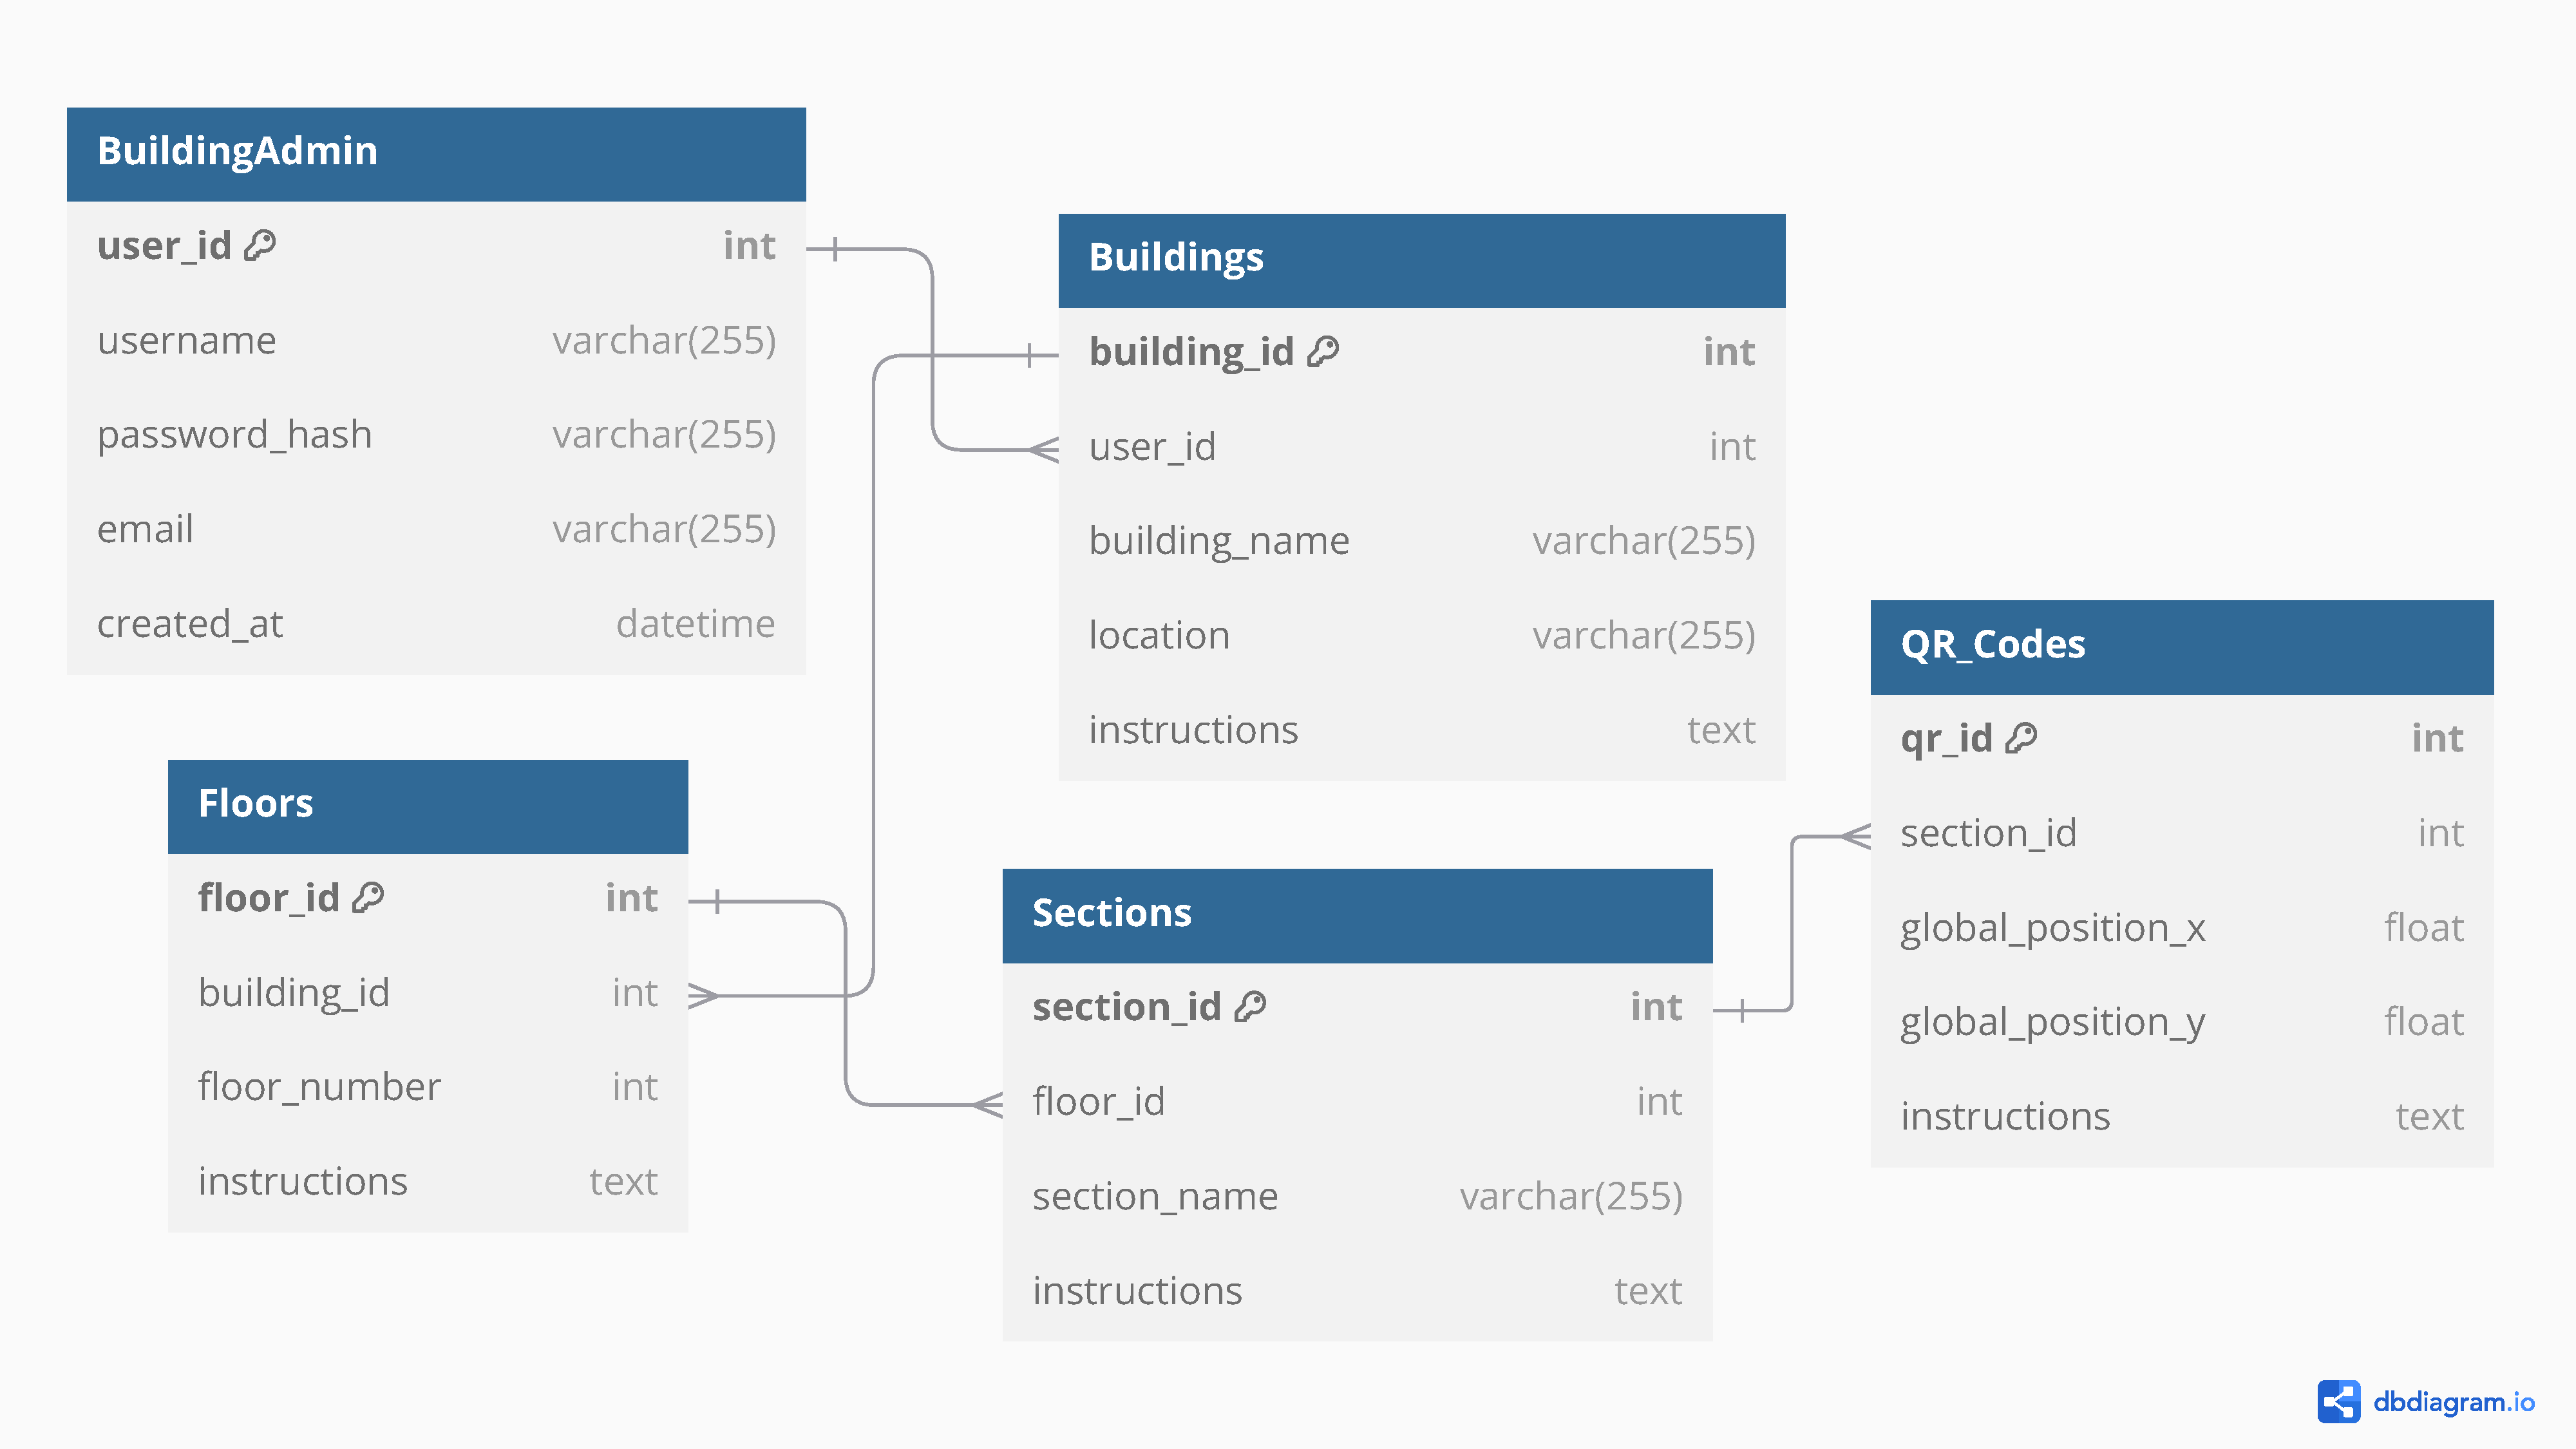
\includegraphics[width=1\linewidth]{assets/ch3/our_ERD}
	\caption{This Entity-Relationship Diagram (ERD) of Mosaned database}
	\label{fig:our_ERD}
\end{figure}

\subsection{Table: BuildingAdmin}  
\begin{itemize}
	\item \textbf{user\_id (Primary Key)}: A unique identifier for each user of the system, enabling individual management of buildings and associated data.
	\item \textbf{username}: The name chosen by the user for login purposes.
	\item \textbf{password\_hash}: A secure hash of the user's password used for authentication.
	\item \textbf{email}: The user's email address, utilized for notifications and account recovery.
	\item \textbf{created\_at}: A timestamp indicating when the user account was created.
\end{itemize}

\subsection{Table: Buildings}  
\begin{itemize}
	\item \textbf{building\_id (Primary Key)}: A unique identifier for each building within the system.
	\item \textbf{user\_id (Foreign Key)}: Links the building to the associated user in the \texttt{BuildingAdmin} table, ensuring that each building is managed by the correct user.
	\item \textbf{building\_name}: The name of the building.
	\item \textbf{location}: The physical address or description of the building's location.
	\item \textbf{instructions}: General instructions related to the building, providing contextual information for navigation and management.
\end{itemize}

\subsection{Table: Floors}  
\begin{itemize}
	\item \textbf{floor\_id (Primary Key)}: A unique identifier for each floor within a building.
	\item \textbf{building\_id (Foreign Key)}: Associates the floor with its corresponding building, establishing a clear hierarchical structure.
	\item \textbf{floor\_number}: Indicates the number of the floor (e.g., 1 for the first floor, 2 for the second, etc.).
	\item \textbf{instructions}: Specific instructions related to that floor, assisting users with effective navigation.
\end{itemize}

\subsection{Table: Sections}  
\begin{itemize}
	\item \textbf{section\_id (Primary Key)}: A unique identifier for each section on a floor.
	\item \textbf{floor\_id (Foreign Key)}: Links the section to its respective floor, maintaining the organizational hierarchy.
	\item \textbf{section\_name}: The name or description of the section within the floor.
	\item \textbf{instructions}: Instructions specific to the section, enhancing the user’s ability to navigate the area.
\end{itemize}

\subsection{Table: QR\_Codes}  
\begin{itemize}
	\item \textbf{qr\_id (Primary Key)}: A unique identifier for each QR code, ensuring no duplicates exist within the system.
	\item \textbf{section\_id (Foreign Key)}: Connects the QR code to its specific section.
	\item \textbf{global\_position\_x}: The X-coordinate representing the global position of the QR code.
	\item \textbf{global\_position\_y}: The Y-coordinate indicating the QR code's position, further aiding in navigation.
	\item \textbf{instructions}: Specific instructions directly linked to the QR code, providing targeted guidance for users when the QR code is scanned.
\end{itemize}




\subsection{Application Programming Interface (API)}

The API serves as the bridge between the mobile app, the database, and the building management dashboard. Its primary responsibilities are:
\begin{itemize}
	\item \textbf{Data Retrieval and Delivery:} When a QR code is scanned, the API retrieves the associated information from the database and sends it to the mobile app for processing.
	\item \textbf{Instruction Updates:} The API also handles data updates from the dashboard, ensuring the latest QR code instructions are accessible to users in real time.
	\item \textbf{User Authentication:} Manages secure access to both the dashboard and the mobile app, allowing only authenticated users to modify or retrieve data.
\end{itemize}

\textcolor{blue}{
	\begin{itemize}
		\item ADD one example of API Endpoints, and the rest on Appendix 
\end{itemize}}

\subsection{Web Server}

The Web Server hosts the building management dashboard and processes web requests, allowing administrators to view and manage QR code data and building layouts. It communicates with the API to send updates to the database and deliver real-time data to the mobile app. 

\textcolor{blue}{
	\begin{itemize}
		\item ADD What tools/framework used to host the dashboard on 3.6
\end{itemize}}


